% TikZ code for KST proof sketch, v22 (granular highlights)
\begin{tikzpicture}[scale=0.8, every node/.style={transform shape, scale=0.8}]
\pgfdeclarelayer{background}\pgfdeclarelayer{main}\pgfsetlayers{background,main}
\coordinate (U0) at (0, 4.0);
\coordinate (U1) at (0, 3.0);
\coordinate (U2) at (0, 2.0);
\coordinate (U3) at (0, 1.0);
\coordinate (U4) at (0, 0.0);
\coordinate (W0) at (4.5, 3.5);
\coordinate (W1) at (4.5, 2.5);
\coordinate (W2) at (4.5, 1.5);
\coordinate (W3) at (4.5, 0.5);
\begin{pgfonlayer}{main}
\uncover<1->{
  \node[draw, thick, fill=yellow!20, rounded corners, align=center, text width=6.5cm] at (2.25, 5.0) {This graph has the maximum number of edges ($|E|=13$) to be $K_{3,2}$-free.};
  \draw[line width=0.7pt, black!25] (U0) -- (W0);
  \draw[line width=0.7pt, black!25] (U0) -- (W1);
  \draw[line width=0.7pt, black!25] (U0) -- (W2);
  \draw[line width=0.7pt, black!25] (U0) -- (W3);
  \draw[line width=0.7pt, black!25] (U1) -- (W0);
  \draw[line width=0.7pt, black!25] (U1) -- (W1);
  \draw[line width=0.7pt, black!25] (U1) -- (W2);
  \draw[line width=0.7pt, black!25] (U2) -- (W0);
  \draw[line width=0.7pt, black!25] (U2) -- (W3);
  \draw[line width=0.7pt, black!25] (U3) -- (W1);
  \draw[line width=0.7pt, black!25] (U3) -- (W3);
  \draw[line width=0.7pt, black!25] (U4) -- (W2);
  \draw[line width=0.7pt, black!25] (U4) -- (W3);
  \fill[black] (U0) circle (2.8pt) node[anchor=east] {$U_{1}$};
  \fill[black] (U1) circle (2.8pt) node[anchor=east] {$U_{2}$};
  \fill[black] (U2) circle (2.8pt) node[anchor=east] {$U_{3}$};
  \fill[black] (U3) circle (2.8pt) node[anchor=east] {$U_{4}$};
  \fill[black] (U4) circle (2.8pt) node[anchor=east] {$U_{5}$};
  \fill[black] (W0) circle (2.8pt) node[anchor=west] {$W_{1}$};
  \fill[black] (W1) circle (2.8pt) node[anchor=west] {$W_{2}$};
  \fill[black] (W2) circle (2.8pt) node[anchor=west] {$W_{3}$};
  \fill[black] (W3) circle (2.8pt) node[anchor=west] {$W_{4}$};
}
\only<2>{
  \fill[brown!40!red] (W1) circle (3.3pt);
  \fill[brown!40!red] (W2) circle (3.3pt);
  \fill[brown!40!red] (U0) circle (3.3pt);
  \fill[brown!40!red] (U1) circle (3.3pt);
  \fill[brown!40!red] (U3) circle (3.3pt);
  \draw[line width=1.0499999999999998pt, brown!40!red, dashed, -] (U3) -- (W2) node[midway, below, sloped, font=\scriptsize] {Add edge};
  \draw[line width=1.0499999999999998pt, brown!40!red] (U0) -- (W1);
  \draw[line width=1.0499999999999998pt, brown!40!red] (U0) -- (W2);
  \draw[line width=1.0499999999999998pt, brown!40!red] (U1) -- (W1);
  \draw[line width=1.0499999999999998pt, brown!40!red] (U1) -- (W2);
  \draw[line width=1.0499999999999998pt, brown!40!red] (U3) -- (W1);
  \node[draw, thick, fill=brown!40!red!20, rounded corners, align=center, text width=6.0cm, overlay] at (2.25, -1.5) {{For example, adding the edge $\{U_4, W_3\}$ creates a $K_{3,2}$ on vertices $\{U_1, U_2, U_4\}$ and $\{W_2, W_3\}$.}};
}
\uncover<3-8>{
  \node[draw, thick, fill=teal!20, rounded corners, align=center, text width=6.0cm, overlay] at (2.25, -1.5) {{For $x=U_1$, we count its $\binom{4}{2}=6$ stars.}};
}
\only<3>{
  \fill[teal] (U0) circle (3.3pt);
  \fill[teal] (W0) circle (3.3pt);
  \fill[teal] (W1) circle (3.3pt);
  \draw[line width=1.0499999999999998pt, teal] (U0) -- (W0);
  \draw[line width=1.0499999999999998pt, teal] (U0) -- (W1);
}
\only<4>{
  \fill[teal] (U0) circle (3.3pt);
  \fill[teal] (W0) circle (3.3pt);
  \fill[teal] (W2) circle (3.3pt);
  \draw[line width=1.0499999999999998pt, teal] (U0) -- (W0);
  \draw[line width=1.0499999999999998pt, teal] (U0) -- (W2);
}
\only<5>{
  \fill[teal] (U0) circle (3.3pt);
  \fill[teal] (W0) circle (3.3pt);
  \fill[teal] (W3) circle (3.3pt);
  \draw[line width=1.0499999999999998pt, teal] (U0) -- (W0);
  \draw[line width=1.0499999999999998pt, teal] (U0) -- (W3);
}
\only<6>{
  \fill[teal] (U0) circle (3.3pt);
  \fill[teal] (W1) circle (3.3pt);
  \fill[teal] (W2) circle (3.3pt);
  \draw[line width=1.0499999999999998pt, teal] (U0) -- (W1);
  \draw[line width=1.0499999999999998pt, teal] (U0) -- (W2);
}
\only<7>{
  \fill[teal] (U0) circle (3.3pt);
  \fill[teal] (W1) circle (3.3pt);
  \fill[teal] (W3) circle (3.3pt);
  \draw[line width=1.0499999999999998pt, teal] (U0) -- (W1);
  \draw[line width=1.0499999999999998pt, teal] (U0) -- (W3);
}
\only<8>{
  \fill[teal] (U0) circle (3.3pt);
  \fill[teal] (W2) circle (3.3pt);
  \fill[teal] (W3) circle (3.3pt);
  \draw[line width=1.0499999999999998pt, teal] (U0) -- (W2);
  \draw[line width=1.0499999999999998pt, teal] (U0) -- (W3);
}
\uncover<9>{
  \node[draw, thick, fill=teal!20, rounded corners, align=center, text width=6.0cm, overlay] at (2.25, -1.5) {{In the example, there are at least $5\binom{13/5}{2} = 10.4$ stars (there are actually 12)}};
}
\uncover<10-12>{
  \node[draw, thick, fill=brown!40!red!20, rounded corners, align=center, text width=6.0cm, overlay] at (2.25, -1.5) {{Each set $T \subset W$ (in this case, $T = \{W_2, W_3\})$ is in at most $s-1 = 3 - 1 = 2$ stars. In total, at most $2 \binom{4}{2}=12$ stars.}};
}
\uncover<11-12>{
  \fill[brown!40!red] (U0) circle (3.3pt);
  \fill[brown!40!red] (W1) circle (3.3pt);
  \fill[brown!40!red] (W2) circle (3.3pt);
}
\uncover<12>{
  \fill[brown!40!red] (U1) circle (3.3pt);
}
\only<11>{
  \draw[line width=1.0499999999999998pt, brown!40!red] (U0) -- (W1);
  \draw[line width=1.0499999999999998pt, brown!40!red] (U0) -- (W2);
}
\only<12>{
  \draw[line width=1.0499999999999998pt, brown!40!red] (U1) -- (W1);
  \draw[line width=1.0499999999999998pt, brown!40!red] (U1) -- (W2);
}
\uncover<13>{
  \node[draw, thick, fill=yellow!20, rounded corners, align=center, text width=6.0cm, overlay] at (2.25, -1.5){{In the example, we conclude that $10.4 \leq 12$, which is true. For bigger values of $z$ this would fail, leading to contradiction and therefore upper bounding $z$. In fact, z=14 already fails! }};
}
\end{pgfonlayer}\end{tikzpicture}